\documentclass{article}

\usepackage{proposal}
\usepackage{caption}

\setproposaltitle{Nonparametric Manifold Clustering for Arbitrary Shaped Clusters}

\setauthor{Sarthak Mittal}{150640}
\addauthor{Gurpreet Singh}{150259}
\addauthor{Debabrata Ghosh}{13817226}

\begin{document}
\makeheader

\rabstract{We study a number of existing techniques that allow clustering of data by jointly representing the data in a low dimensional latent form and performing clustering over this latent space. The key idea in such models is that the given data can be generated from a simpler pattern in a possibly lower-dimensional manifold through some non-linear mapping. Using a nonparametric clustering model over a latent space and a good approximation function that maps the latent space to our data space, it is possible to infer both, the number of clusters that the data lies in, and the varied shapes of the clusters in the data. Moreover, we try to come up with a model that not only performs this task efficiently but is also able to scale to large amounts of data.}

\begin{psection}{Problem}
In this course project, we aim to solve the problem of uncovering both the number of clusters and their arbitrary shapes. Moreover, we aim to propose a model that not only solves the above problem efficiently, but also scales up with the amount of data without requiring massive computational costs. To successfully come up with a solution to the problem, we start with a background reading of the concepts required and the existing work done in this context. Further, we propose the general framework of our model and provide reasons for its probable effectiveness over the previous models.
\end{psection}

\begin{psection}{Introduction}

	Humans are capable of recognizing cluster patterns even when the shapes and sizes of the clusters are immensely varied. The intrinsic shortcomings of K-Means and Gaussian Mixture Models are that the model needs the number of clusters to be specified before-hand and is able to cluster the data in only Gaussian shaped clusters. Though Dirichlet Process Mixture Models alleviate the former problem of the model, it still tries to capture the data as a cluster of Gaussians.

	One of the most popular ways to solve this problem is by constructing a latent representation of the data and a complex non-linear function that can efficiently map the latent space representations to the data space representations. The latent representation can be thought of as a simple distribution like a mixture of Gaussians which is warped by a complex non-linear function to represent the data. Now, clustering on this latent representation by models that only allow gaussian-like cluster shapes still allow for arbitrary shaped clusters in the data space because of the non-linear warping function.

	One way to do the above problem is to first uncover a good latent representation of the data through some non-linear transformation techniques like a Gaussian Process variant of Probabilistic Principal Component Analysis or through a Variational Autoencoder. Both of these constitute powerful non-linear function approximators and thus solve the problem well. Once we have the latent representation of the data, we perform clustering on the latent representation through some standard clustering techniques like Gaussian Mixture Model or Dirichlet Process Mixture Model. Thus, we get clusters of arbitrary shapes.

	The above technique, however, is not optimal because in doing so, we have made the task of latent representation and clustering mutually independent. However, we can see that these tasks are actually quite related to each other and any model would be able to construct more disambiguated latent representations if it performs the task of latent representation and clustering jointly. Thus, to efficiently solve the problem, we define a Generative Model where a vector in the latent space is sampled from a mixture of Gaussians (either a finite mixture of an infinite mixture) and then learn a complex non-linear function that maps the latent space to data space.

\end{psection}

\begin{psection}{Relevant Background}

\begin{psubsection}{Gaussian Process}

	Gaussian Processes or GPs define non-parametric distributions over non-linear functions.
	A GP, denoted as $\tfunc{GP}{\vmu, \Sigma}$ is defined as by a \et{mean function} $\vmu$ and a \et{covariance function} $\Sigma$. A function $f : \bR^D \ra \bR$, sampled from a Gaussian Process is written as
	\begin{align*}
		\vf	\qsim	\tfunc{GP}{\vmu, \Sigma}
	\end{align*}

	We can imagine a function to be an infinite dimensional vector. Therefore, essentially GP samples infinite dimensional vectors, \ie random function $\vf$.

	More formally, a GP can be thought of as a Stochastic Process defined in such a way that any finite-dimensional subset $\set{x_n \in \bR}_{n = 1}^N$ of the infinite-dimensional vector is distributed as a Gaussian Distribution. Thus, a GP assumes that the distribution $\prob{f(x_1), f(x_2) \dots f(x_N)}$ is jointly a multivariate gaussian, with some mean $\vmu(\vX) \in \bR^N$ and some $\Sigma(\vX) \in \bR^{N \times N}$, where $X = \set{\vx_n}_{n = 1}$ \citep{murphy}.

	\note{For the ease of notation, we define $\vf = \tr{\brac{f(\vx_1), f(\vx_2) \dots f(\vx_N)}}$}

	Therefore, a Gaussian Process generalizes the underlying distribution of a function $f : \bR^D \ra \bR$. That is, given a set of points $\set{x_n \in \bR^D}_{n = 1}^N$ and their respective mappings $\set{f^\ast{(x_n)}}_{n = 1}^N$, it is possible to model probable continuous functions representing $f^\ast$ using a GP. We denote this as following
	\begin{align*}
		\vf			&\qsim	\tfunc{GP}{\vmu(\vX), \Sigma(\vX)} \\
	\intertext{where}
		\vmu(\vX)	&\eq	\E{\vf} \\
		\Sigma(\vX)	&\eq	\E{\tr{\para{\vf - \vmu(X)}} \para{\vf - \vmu(X)}}
	\end{align*}

	The covariance matrix specifies the smoothness of the function sampled using a GP.
	In fact, each entry of the covariance matrix is the similarity between the respective pair of points, \ie $\Sigma_{(i, j)} = \kappa(\vx_i, \vx_j)$ where $\kappa$ is a kernel \citep[see][]{kernel} or similarity function.

	We can alternatively say that $\vf$ is sampled from a Gaussian Process $\tfunc{GP}{\vmu, \Sigma}$, if its finite dimensional marginal is jointly a multivariate distribution. More formally, $\vf \sim \tfunc{GP }{\vmu, \Sigma}$ if for all $N \in \bN$ and any arbitrary set of points $\set{\vx_n}_{n = 1}^N$, we have
	\begin{align*}
		\brac{\begin{matrix}
			f(\vx_1) \\
			f(\vx_2) \\
			\vdots \\
			f(\vx_N)
		\end{matrix}}
		\eq	\ND{
			\brac{\begin{matrix}
					\vmu(\vx_1) \\
					\vmu(\vx_2) \\
					\vdots \\
					\vmu(\vx_N)
			\end{matrix}},
			\brac{\begin{matrix}
					\kappa(\vx_1, \vx_1)	&	\kappa(\vx_1, \vx_2)	&	\dots	&	\kappa(\vx_1, \vhx_N)	\\
					\kappa(\vx_2, \vx_1)	&	\kappa(\vx_2, \vx_2)	&	\dots	&	\kappa(\vx_2, \vx_N)	\\
					\vdots 					&	\vdots	 			&	\vdots	&	\vdots				\\
					\kappa(\vx_N, \vx_1)	&	\kappa(\vx_N, \vx_2)	&	\dots	&	\kappa(\vx_N, \vx_N)
			\end{matrix}}
		}
	\end{align*}

	It is noteworthy that all marginals or conditionals for the random vectors are Gaussian distributions as per Gaussian properties \footnote{Any subset of $\vf$ will be a random vector, which in case of Gaussian Processes will be a Gaussian Distribution itself}.
%	Also, a GP is conjugate to itself.
%	This is because they are represented by multivariate gaussian distributions, and therefore follow all the properties of gaussian distributions.

	This makes Gaussian processes very interesting to study, and also easily applicable in a wide variety of tasks, such as non-linear regression and classification.
	Another application of Gaussian Processes is in latent representation of high-dimensional vectors for clustering purposes \citep{gplvm}, which is discussed in \hyperlink{subsec:2.4}{4.1}.

\end{psubsection}

\begin{psubsection}{Dirichlet Process Mixture Models}

	Similar to Gaussian Processes, Dirichlet Processes or DPs are a family of stochastic processes.
	A Dirichlet process defines a distribution over probability measures $G : \Theta \ra \bR^+$, where, for any finite partition of $\Theta$, say $\set{\vtheta_k}_{k = 1}^K$, the random vector $\para{G(\vtheta_1), G(\vtheta_2) \dots G(\vtheta_K)}$ is jointly generalized under a Dirichlet Distribution \citep{murphy} \footnote{G(\vtheta) is random since $G$ itself is random and is sampled from the Dirichlet Process}, written as
	\begin{align*}
		\para{G(\vtheta_i), G(\vtheta_2) \dots G(\vtheta_K)}	\qsim	\tfunc{Dir}{\alpha G_0(\vtheta_1), \alpha G_0(\vtheta_2) \dots \alpha G_0(\vtheta_K)}
	\end{align*}
	where $\alpha$ is called the concentration parameter and $G_0$ is the base distribution. $\alpha G_0$ collectively is called the base measure.

	Dirichlet processes are particularly useful in the task of non-parametric approach clustering, using a mixture of Dirichlet Processes \citep{dp-ferg, dp-anto} (commonly DP Mixture Models or Infinite Mixture Models).
	In fact, a DP Mixture Model can be seen as an extension of Gaussian Mixture Models over a non-parametric setting.

	The basic DP Mixture Model follows the following generative story
	\begin{align*}
		\mdef{Likelihood}			\vy_n \pipe \vtheta_n	&\qsim	F(\vy_n \pipe \vtheta_n) & \\
		\mdef{Conditional Prior}	\vtheta \pipe G			&\qsim	G \\
		\mdef{Hyperparameter}				G						&\qsim	\tfunc{DP}{G_0, \alpha}
	\end{align*}
	where $G \sim$ DP denotes sampling from a Dirichlet Process given a base measure.

	When we are dealing with DP Mixture Models for clustering, it helps to integrate out $G$ with respect to the prior on $G$. \citep{neal}. Therefore, we can write the clustering problem in an alternate representation, although the underlying model remains the same.
	\begin{align*}
		\mdef{Likelihood}			\vy_n \pipe c_n, \Phi	&\qsim	F(\vy_n \pipe \vphi_{c_n}) & \\
		\mdef{Latent Distribution}	c_n \pipe \vp			&\qsim	\tfunc{Discrete}{p_1, p_2 \dots p_K} \\
		\mdef{Priors}				\vphi_k					&\qsim	G_0 & \\
		&&							\vp						&\qsim	\tfunc{Dir}{p_1, p_2 \dots p_K}
	\end{align*}
	where $c_n$ is the cluster assignment for the $n$\tth point and $\Phi = \set{\vphi_k}_{k = 1}^{K}$ are the likelihood parameters for each cluster. $K$ denotes the number of clusters, and being a non-parametric model, we assume $K \ra \infty$.

	If the likelihood and the base distribution are conjugate, we can easily derive a posterior representation for the cluster assignments or the latent classes, and use inference techniques such as Mean Field VB \citep{blei} and Monte Carlo Markov Chain \citep{esc-west, neal}.	\et{Neal} also describes various inference methods in case of non-conjugate base distribution.

	Dirichlet processes are extremely useful for clustering purposes as they do not assume an inherent base distribution, and therefore it is possible to apply Dirichlet Process priors over complex models.

\end{psubsection}

\begin{psubsection}{Variational Autoencoder}

    Variational autoencoders (VAEs) are essentially a deep learning technique for learning latent representations. We can consider a directed latent-variable model of the form
    \begin{align*}
        \vp(\vx,\vz)=\vp(\vx|\vz)\vp(\vz)
    \end{align*}
    with observed $\vx \in \mathcal{X}$, where $\mathcal{X}$ can be continuous, discrete, or latent. Suppose that given a dataset $\mathbb{D}= \{x^1,\ldots,x^n\}$, we may be interested in the following inference and learning tasks:
    \begin{itemize}
        \item Learning the parameters $\theta$ of $\vp$.
        \item Approximate posterior inference over $\vz$.
        \item Approximate marginal inference over $\vx$.
    \end{itemize}

    Auto-encoding variational Bayes (AEVB) is an algorithm that can efficiently solve these three inference and learning tasks; the variational auto-encoder being one instantiation of this algorithm. In variational inference, we are interested in maximizing the evidence lower bound (ELBO)
    \begin{align*}
        \mathcal{L}(\vp_\theta,\vq_\phi)=\mathbb{E}_{\vq_\phi(\vz|\vx)}[\text{log } \vp_\theta(\vx,\vz)-\text{log } \vq_\phi(\vz|\vx)]
    \end{align*}
    over the space of whole $\vq_\phi$ and evidently satisfies the equation
    \begin{align*}
        \text{log } \vp_\theta(\vx)= \mathbb{KL}[\vq_\phi(\vz|\vx)||\vp_\theta(\vz|\vx)]+\mathcal{L}(\vp_\theta,\vq_\phi)
    \end{align*}
    Since $\vx$ is fixed, we can define $\vq_\phi(\vz|\vx)$ to be conditioned on $\vx$ meaning that we are effectively choosing a different $\vq(\vz)$ for every $\vx$, which will produce a better posterior approximation than always choosing the same $\vq(\vz)$. Now the question is how we optimize over $\vq(\vz|\vx)$?

    One approach called black-box variational inference consists of maximizing the ELBO using gradient descent over $\phi$ only assuming that $\vq_\phi$ is differentiable in its parameters $\phi$ which involves computing the gradient
    \begin{align*}
        \nabla_{\theta,\phi} \mathbb{E}_{\vq_\phi(\vz)}[\text{log } \vp_\theta(\vx,\vz)-\text{log } \vq_\phi(\vz)]
    \end{align*}
    One way to estimate this gradient is via the so-called score function estimator:
    \begin{align*}
        \nabla_{\phi} \mathbb{E}_{\vq_\phi(\vz)}[\text{log } \vp_\theta(\vx,\vz)-\text{log } \vq_\phi(\vz)] =
        \mathbb{E}_{\vq_\phi(\vz)}[(\text{log } \vp_\theta(\vx,\vz)-\text{log } \vq_\phi(\vz))\nabla_{\phi}\text{log } \vq_\phi(\vz)]
    \end{align*}
    which follows from some basic algebra and calculus \citep{Mnih}.

    The above identity referred to as score function estimator places the gradient inside the expectation, which we may now evaluate using Monte Carlo. Unfortunately, the score function estimator has an important shortcoming: it has a high variance. The key contribution of the VAE paper \citep{VAE} is to propose an alternative estimator that is much better behaved which is done in two steps: we first reformulate the ELBO so that parts of it can be computed in closed form (without Monte Carlo), and then we use an alternative gradient estimator, based on the so-called \textit{reparametrization trick}.

    By rearranging the ELBO we get the reformulation called SGVB estimator as follows:
    \begin{align*}
        \text{log } \vp(x) \geq \mathbb{E}_{\vq_\phi(\vz|\vx)}[\text{log } \vp_\theta(\vx|\vz)]-\mathbb{KL}[\vq_\phi(\vz|\vx)||\vp(\vz)]
    \end{align*}

    We may think of $\vx$ as an observed data point. The left-hand side consists of two terms, both of which involve taking a sample $\vz \sim \vq_\phi(\vz|\vx)$, which we can interpret as a code describing $\vx$. So we refer to $\vq$ as the \textit{encoder}.

    In the first term, $\text{log } \vp_\theta(\vx|\vz)$ is the log-likelihood of the observed $\vx$ given the encoding $\vz$ that we have sampled. This term is maximized when $\text{log } \vp_\theta(\vx|\vz)$ assigns high probability to the original $\vx$. So the attempt is to reconstruct $\vx$ given the encoding $\vz$. Hence we call $\text{log } \vp_\theta(\vx|\vz)$ the \textit{decoder} and the term is called the \textit{reconstruction error}.

    The second term is the divergence between $\vq_\phi(\vz|\vx)$ and the prior $\vp(\vz)$, which we will fix to be $\mathcal{N}(0,\vI)$. It encourages the encodings $\vz$ to look Gaussian. We call it the regularization term. It prevents $\vq_\phi(\vz|\vx)$ from encoding the distribution in arbitrary space and instead forces it to stay close to the prior distribution, so that at test time when we sample from this prior, we indeed get good results.

    Now we can talk about the reparametrization trick to get a low-variance gradient estimator for optimizing our objective. Under certain mild conditions, we may express the distribution $\vq_\phi(\vz|\vx)$ as the following two-step generative process:
    \begin{center}
        First, we sample a noise variable $\epsilon$ from a simple distribution like the standard Normal\\ $\epsilon\sim\mathcal{N}(0,\vI)$\\
        Then, we apply a deterministic transformation $\vh_\phi(\epsilon,\vx)$ that maps the random noise into a more complex distribution\\
        $\vz=\vh_\phi(\epsilon,\vx)$.
    \end{center}
    Gaussian variables provide the simplest example of the reparametrization trick. Given $\mu$ and $\Sigma$ as the mean and covariance of $\vq_\phi(\vz|\vx)$, we can sample from $\mathcal{N}(\mu,\Sigma)$ by first sampling  $\epsilon\sim\mathcal{N}(0,\vI)$ and then computing $\vz=\mu+\Sigma^{\frac{1}{2}}\epsilon$. The biggest advantage of this approach is that we many now write the gradient of an expectation with respect to $\vq_\phi(\vz)$(for any $f$) as
    \begin{align*}
        \nabla_\phi \mathbb{E}_{\vz\sim\vq_\phi(\vz|\vx)} [f(\vx,\vz)] = \nabla_\phi \mathbb{E}_{\epsilon\sim\mathcal{N}(0,\vI)}[f(x,\vh_\phi(\epsilon,\vx))] = \mathbb{E}_{\epsilon\sim\mathcal{N}(0,\vI)}[\nabla_\phi f(x,\vh_\phi(\epsilon,\vx))]
    \end{align*}
    The gradient is now inside the expectation and we may use Monte Carlo to get an estimate of the right-hand term. Still, we have not specified the exact form of $\vp$ or $\vq$ besides saying that these could be arbitrary functions. The best $\vq_\phi(\vz|\vx)$ should be able to approximate the true posterior $\vp(\vz|\vx)$). Similarly, $\vp(\vx)$ should be flexible enough to represent the richness of the data. Therefore, we are going to parameterize $\vp$ and $\vq$ by neural networks.
\end{psubsection}
\end{psection}
\begin{psection}{Related Work}
\begin{psubsection}{Manifold Clustering through GPLVMs}

	\hypertarget{subsec:2.4}{The} model assumes that each observation in some data space has coordinates in a latent space and was generated through some non-linear functional mapping from the latent space to the data space. To tackle the problem of manifold clustering for arbitrary shaped clusters, the infinite Warped Mixture Model (iWMM) \citep{gplvm} assumes that the latent coordinates are generated from a Dirichlet Process Mixture Model and these coordinates are mapped to the observations in data space through some complex non-linear function which is modeled using a Gaussian Process.

	More concretely, assume that we have a data space $\mathbb{R}^K$ and the corresponding latent space $\mathbb{R}^D$. Then the iWMM model defines the following generative story:

	\begin{enumerate}
		\item Draw mixture weights $\vpi \sim Gem(\eta)$
		\item {For each component  c $= 1,...,\infty$
				\begin{enumerate}
					\item Draw precision matrix $\vLambda_c \sim \mathcal{W}(\vS^{-1}, \nu)$
					\item Draw mean vector $\vmu_c \sim \mathcal{N}(\vu, (r\vLambda_c)^{-1})$
			\end{enumerate}}
		\item {For each observed dimension k $=1,...,K$
				\begin{enumerate}
					\item Draw function $f_k(x) \sim GP(m(\vx),k(\vx,\vx'))$
			\end{enumerate}}
		\item For each obsevation n $= 1,...,N$
				\begin{enumerate}
					\item Draw latent cluster assignment $z_n \sim Mult(\vpi)$
					\item Draw latent coordinates $\vx_n \sim \mathcal{N}(\vmu_{z_n},\vLambda_{z_n}^{-1})$
					\item For each observed dimension d = $1,...,D$
						\begin{enumerate}
							\item Draw feature $y_{nd} \sim \mathcal{N}(f_k(\vx_n),\beta^{-1})$
						\end{enumerate}
			\end{enumerate}
	\end{enumerate}

	Note that the $Gem(\pi)$ defines the stick-breaking process that generates mixture weights for a Dirichlet process with parameter $\eta$. Also note that $Mult(\pi)$ defines a Multinomial distribution with parameter $\pi$ and $m(x)$ and $k(x,x')$ are the mean and kernel functions of the Gaussian Process respectively.

	Since the model uses Gaussian Process and Dirichlet Process to jointly learn latent representations and arbitrary shaped clusters, the inference scheme in the procedure is non exact and non trivial. Inference in accomplished through a Sampling based approximate inference scheme, the general structure of which is:

	\begin{enumerate}
		\item For each observation n $= 1,...,N$, sample the cluster assignment $z_n$ by Collapsed Gibbs Sampling
		\item Sample latent coordinates $X$ and kernel parameters using Hybrid Monte Carlo
	\end{enumerate}

	Thus, by constructing a latent manifold on which the data exists and learning a complex non-linear function, the model is able to both accurately uncover clusters and estimate density of the data even when the shapes of the clusters are very varied and non-Gaussian like. The disadvantage of this problem, though, is that since the model uses Gaussian process and Sampling scheme for inference, the complexity of the model increases with the amount of data we have, and thus inference is performed with the comlpexity of each iteration being $\mathcal{O}(N^3)$. Thus, though the model is very powerful, it doesn't scale well.

\end{psubsection}

\begin{psubsection}{Manifold Clustering through GMM-SVAE}
Though the iWMM model is very efficient at uncovering the number of clusters and the cluster shapes, it does not scale well to large amounts of data. To solve this issue, GMM-SVAE \citep{svae} defines the required non-linear functional mapping through a neural network, which have been proved to be universal function approximators. The model takes advantage of the fact that Variational Autoencoders work well in problems of density estimation and hence, on combining VAEs with GMM, the model is able to uncover arbitrary shaped clusters.

In more precise terms, assuming our latent representation of the data lies in $\mathbb{R}^K$ space and our data lies in $\mathbb{R}^D$ space, the model defines the following generative story:

\begin{enumerate}
    \item Draw mixture weights $\vpi \sim Dir(\valpha)$
    \item For each component k $= 1,...,K$
    \begin{enumerate}
        \item Draw $(\vmu_k,\vSigma_k) \sim NIW(\vlambda)$
    \end{enumerate}
    \item Draw parameters of encoder and decoder model $\vgamma \sim p(\vgamma)$
    \item For each observation n = $ 1,...,N$
    \begin{enumerate}
        \item Draw cluster assignment $c_n \sim Mult(\vpi)$
        \item Draw latent coordinates $\vx_n \sim \mathcal{N}(\vmu_{c_n}, \vSigma_{c_n})$
        \item Draw a data point $\vy_n \sim \mathcal{N}(\vmu(\vx_n ; \vgamma), \vSigma(\vx_n;\vgamma)) $
    \end{enumerate}
\end{enumerate}

Note that $Dir(\valpha)$ defines a Dirichlet distribution over the mixing proportions and $NIW(\vlambda)$ defines Normal-Inverse-Wishart distributions over the parameters associated with each cluster. Moreover, $p(\vgamma)$ defines the distribution over the parameters of the encoder-decoder model and $\vmu(\vx_n;\vgamma)$ and $\vSigma(\vx_n;\vgamma)$ are neural networks with parameters $\vgamma$ which map $\vx_n$ to the observed data $\vy_n$.

The model performs inference by using recognition networks to produce local evidence potentials which are then incorporated in the general graphical model inference algorithm that sits on top. It uses a conditional random field (CRF) variational family and learns recognition networks that output conjugate graphical model potentials instead of complete variational distribution's parameters. These potentials are then used in the graphical model inference algorithms in place of non-conjugate likelihoods.

The disadvantage of the model is that it has been worked on only in the parametric setting where the number of clusters present in the data is provided to the network. Hence, though the model efficiently learns the shapes of the clusters, it doesn't give us the number of clusters present in the data. At the same time, it is worth pointing out that this model, through the use of Neural Networks, scales up to increasing amounts of data very efficiently.
\end{psubsection}
\end{psection}

\begin{psection}{DPMM-SVAE}
Our aim is to come up with a model that not only recovers the complex shaped clusters in the data, but also the number of clusters present. Moreover, it should scale well to large amounts of data. To solve this problem, we propose a model similar to the GMM-SVAE model described above. However, instead of having a finite mixture model at the prior like the GMM-SVAE model, we propose to have a Dirichlet Process Mixture Model sitting at the top. This allows creating of new clusters as more and more data is seen.

To achieve this aim, we describe the following generative story:

	\begin{enumerate}
		\item Draw mixture weights $\vpi \sim Gem(\eta)$
		\item {For each component  c $= 1,...,\infty$
			\begin{enumerate}
			    \item Draw $(\vmu_k,\vSigma_k) \sim NIW(\vlambda)$
			\end{enumerate}}
		\item Draw parameters of the encoder and decoder model $\vgamma \sim p(\vgamma)$
		\item For each obsevation n $= 1,...,N$
				\begin{enumerate}
					\item Draw latent cluster assignment $c_n \sim Mult(\vpi)$
					\item Draw latent coordinates $\vx_n \sim \mathcal{N}(\vmu_{c_n},\vLambda_{z_n}^{-1})$
					\item Draw a data point $\vy_n \sim \mathcal{N}(\vmu(x_n;\vgamma),\vSigma(x_n;\vgamma))$
			\end{enumerate}
	\end{enumerate}
Note that while computationally creating an infinite number of clusters is not possible, we solve this problem by using a $Gem(\cdot)$ distribution which describes a stick breaking scheme, where we generate new clusters on demand. Thus, our proposed model is theoretically able to capture both the number of clusters in the data as well as their arbitrary shapes, while being able to scale to large data. Thus, it has the capacity to, in theory, surpass the existing methods mentioned above.
\end{psection}
%\begin{psection}{Inference}
%\end{psection}

\begin{psection}{Experiments}

	\begin{psubsection}{Clustering using Standard GMM and K-Means}

		\begin{figure}[H]
			\captionsetup{justification=centering,margin=0.8cm}
			\centering
			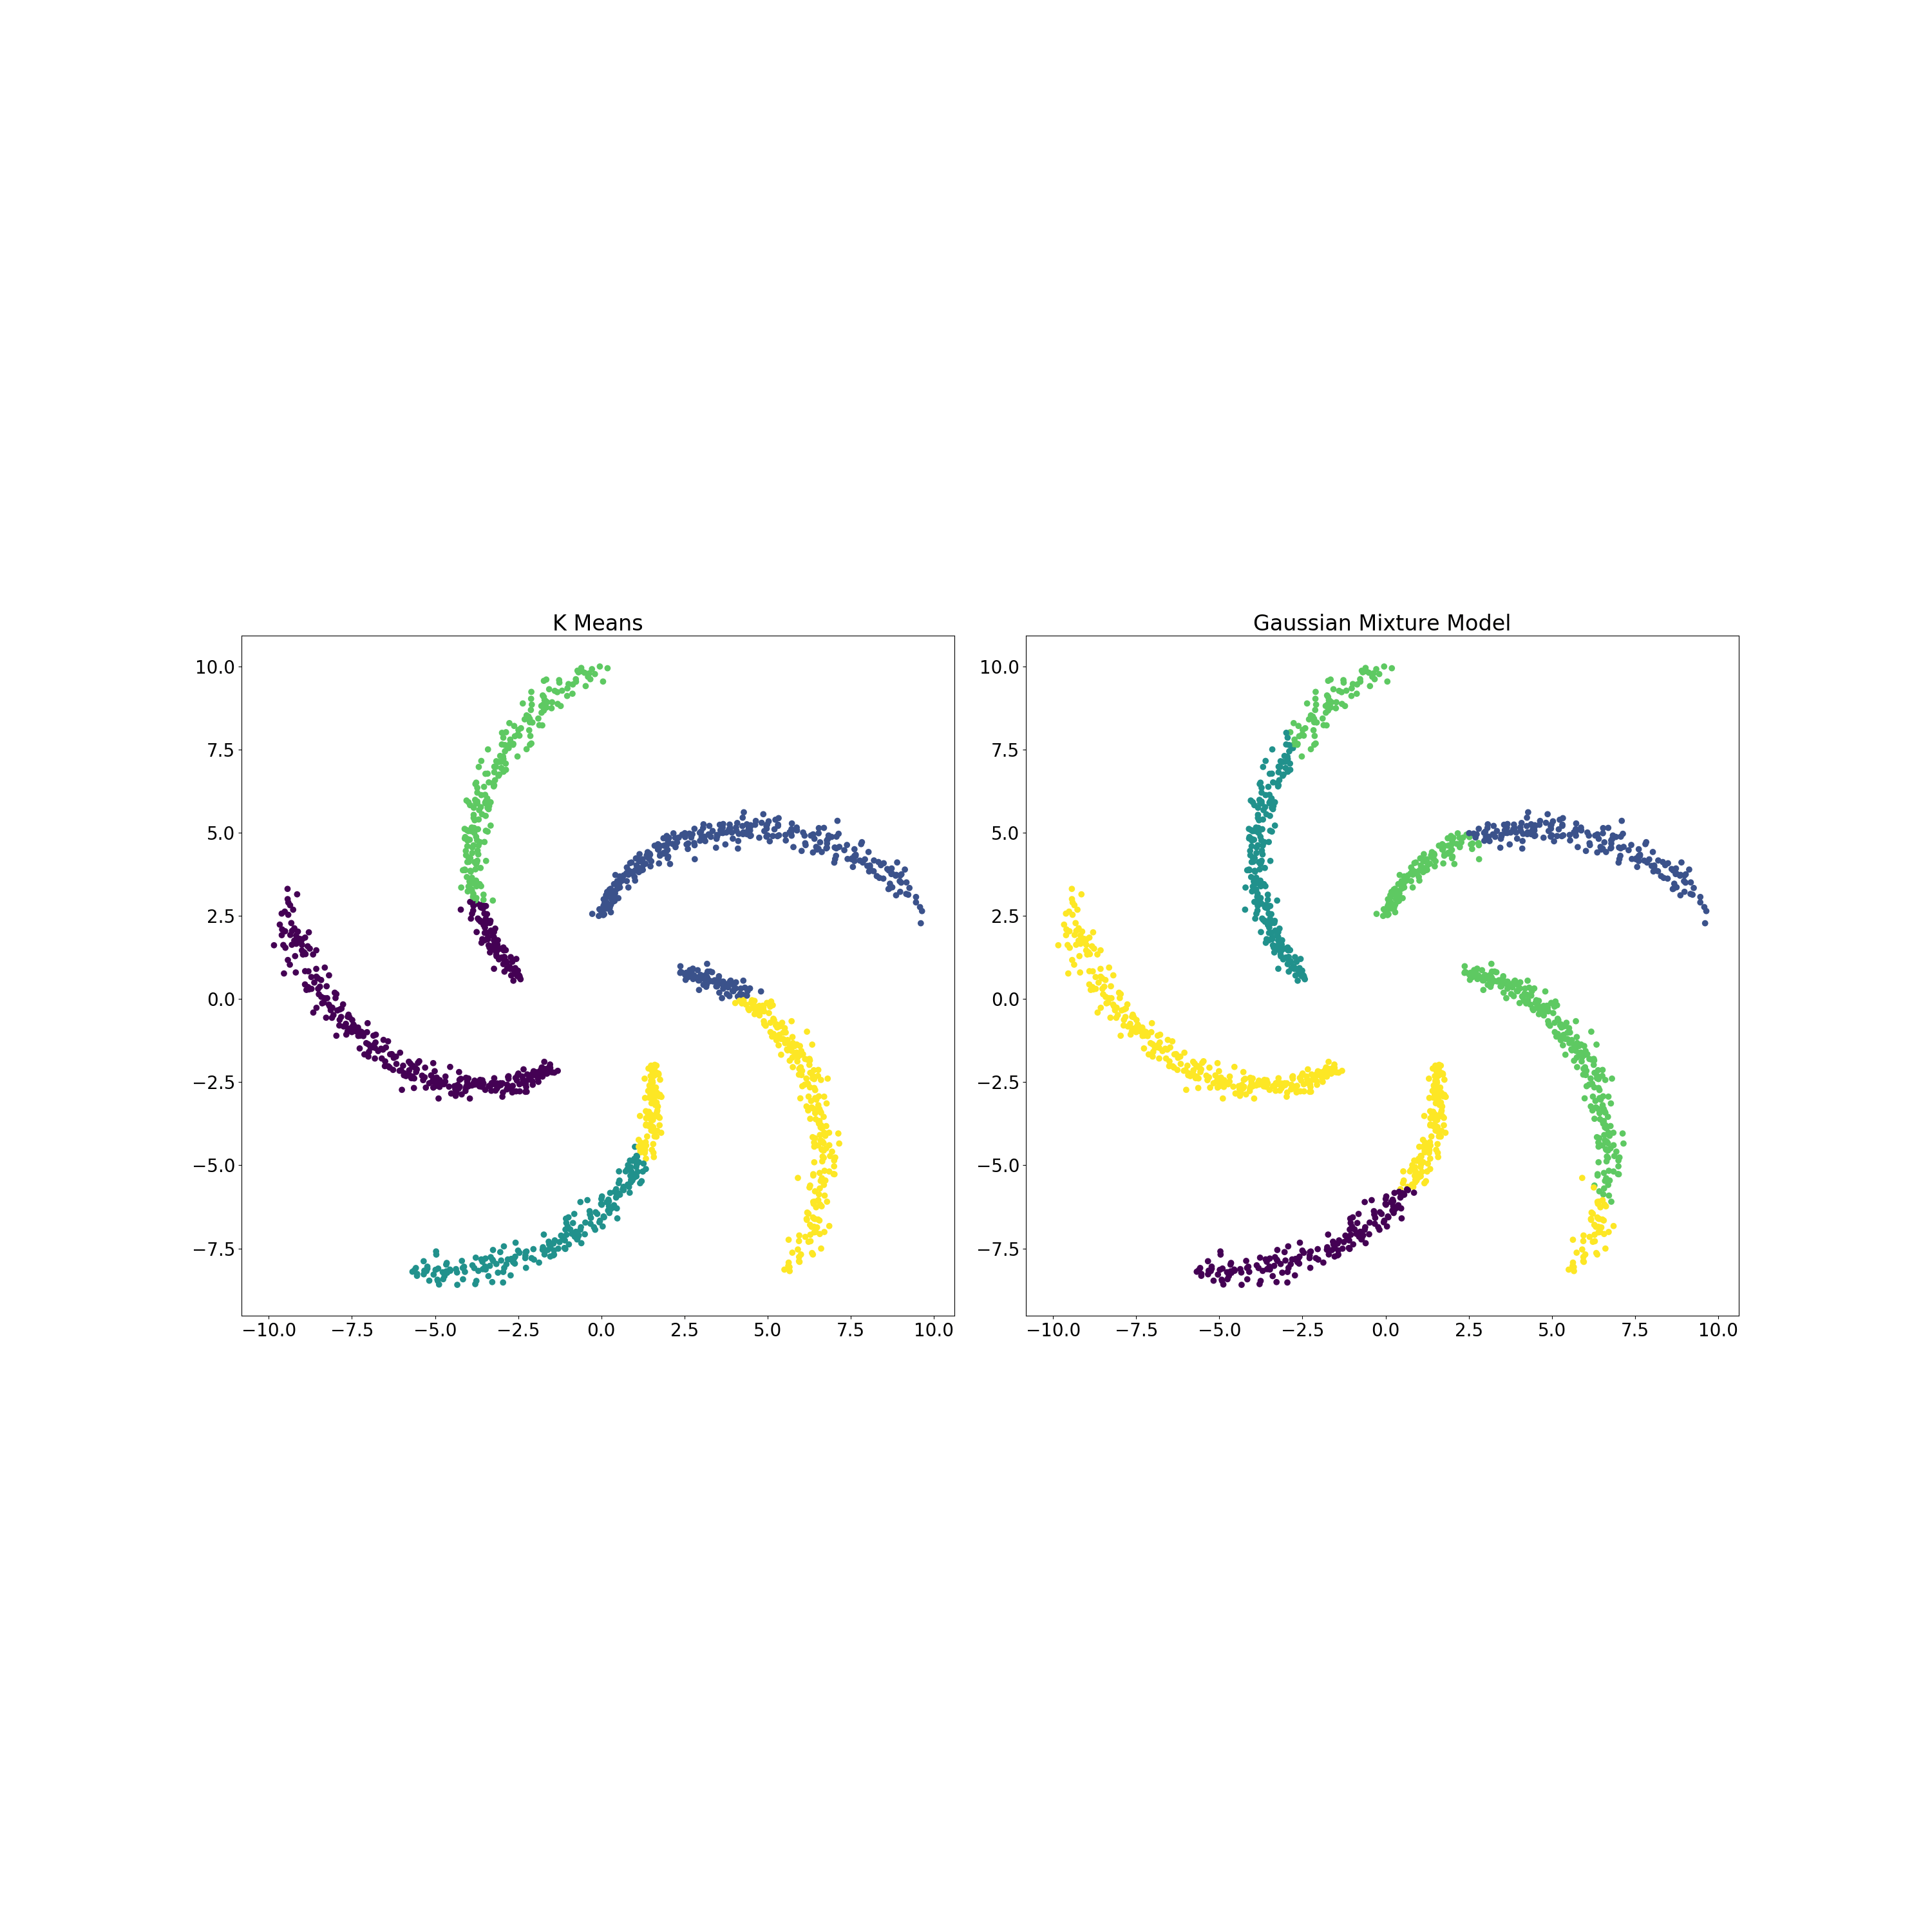
\includegraphics[trim={5cm 32cm 0 34cm},clip,scale=0.14]{includes/clustering.png}
			\caption*{Clustering Spiral Dataset using K-Means and GMM}
		\end{figure}

	\end{psubsection}

	\begin{psubsection}{Clustering on Latent Representation in VAE}

		\begin{figure}[H]
			\captionsetup{justification=centering,margin=0.8cm}
			\centering
			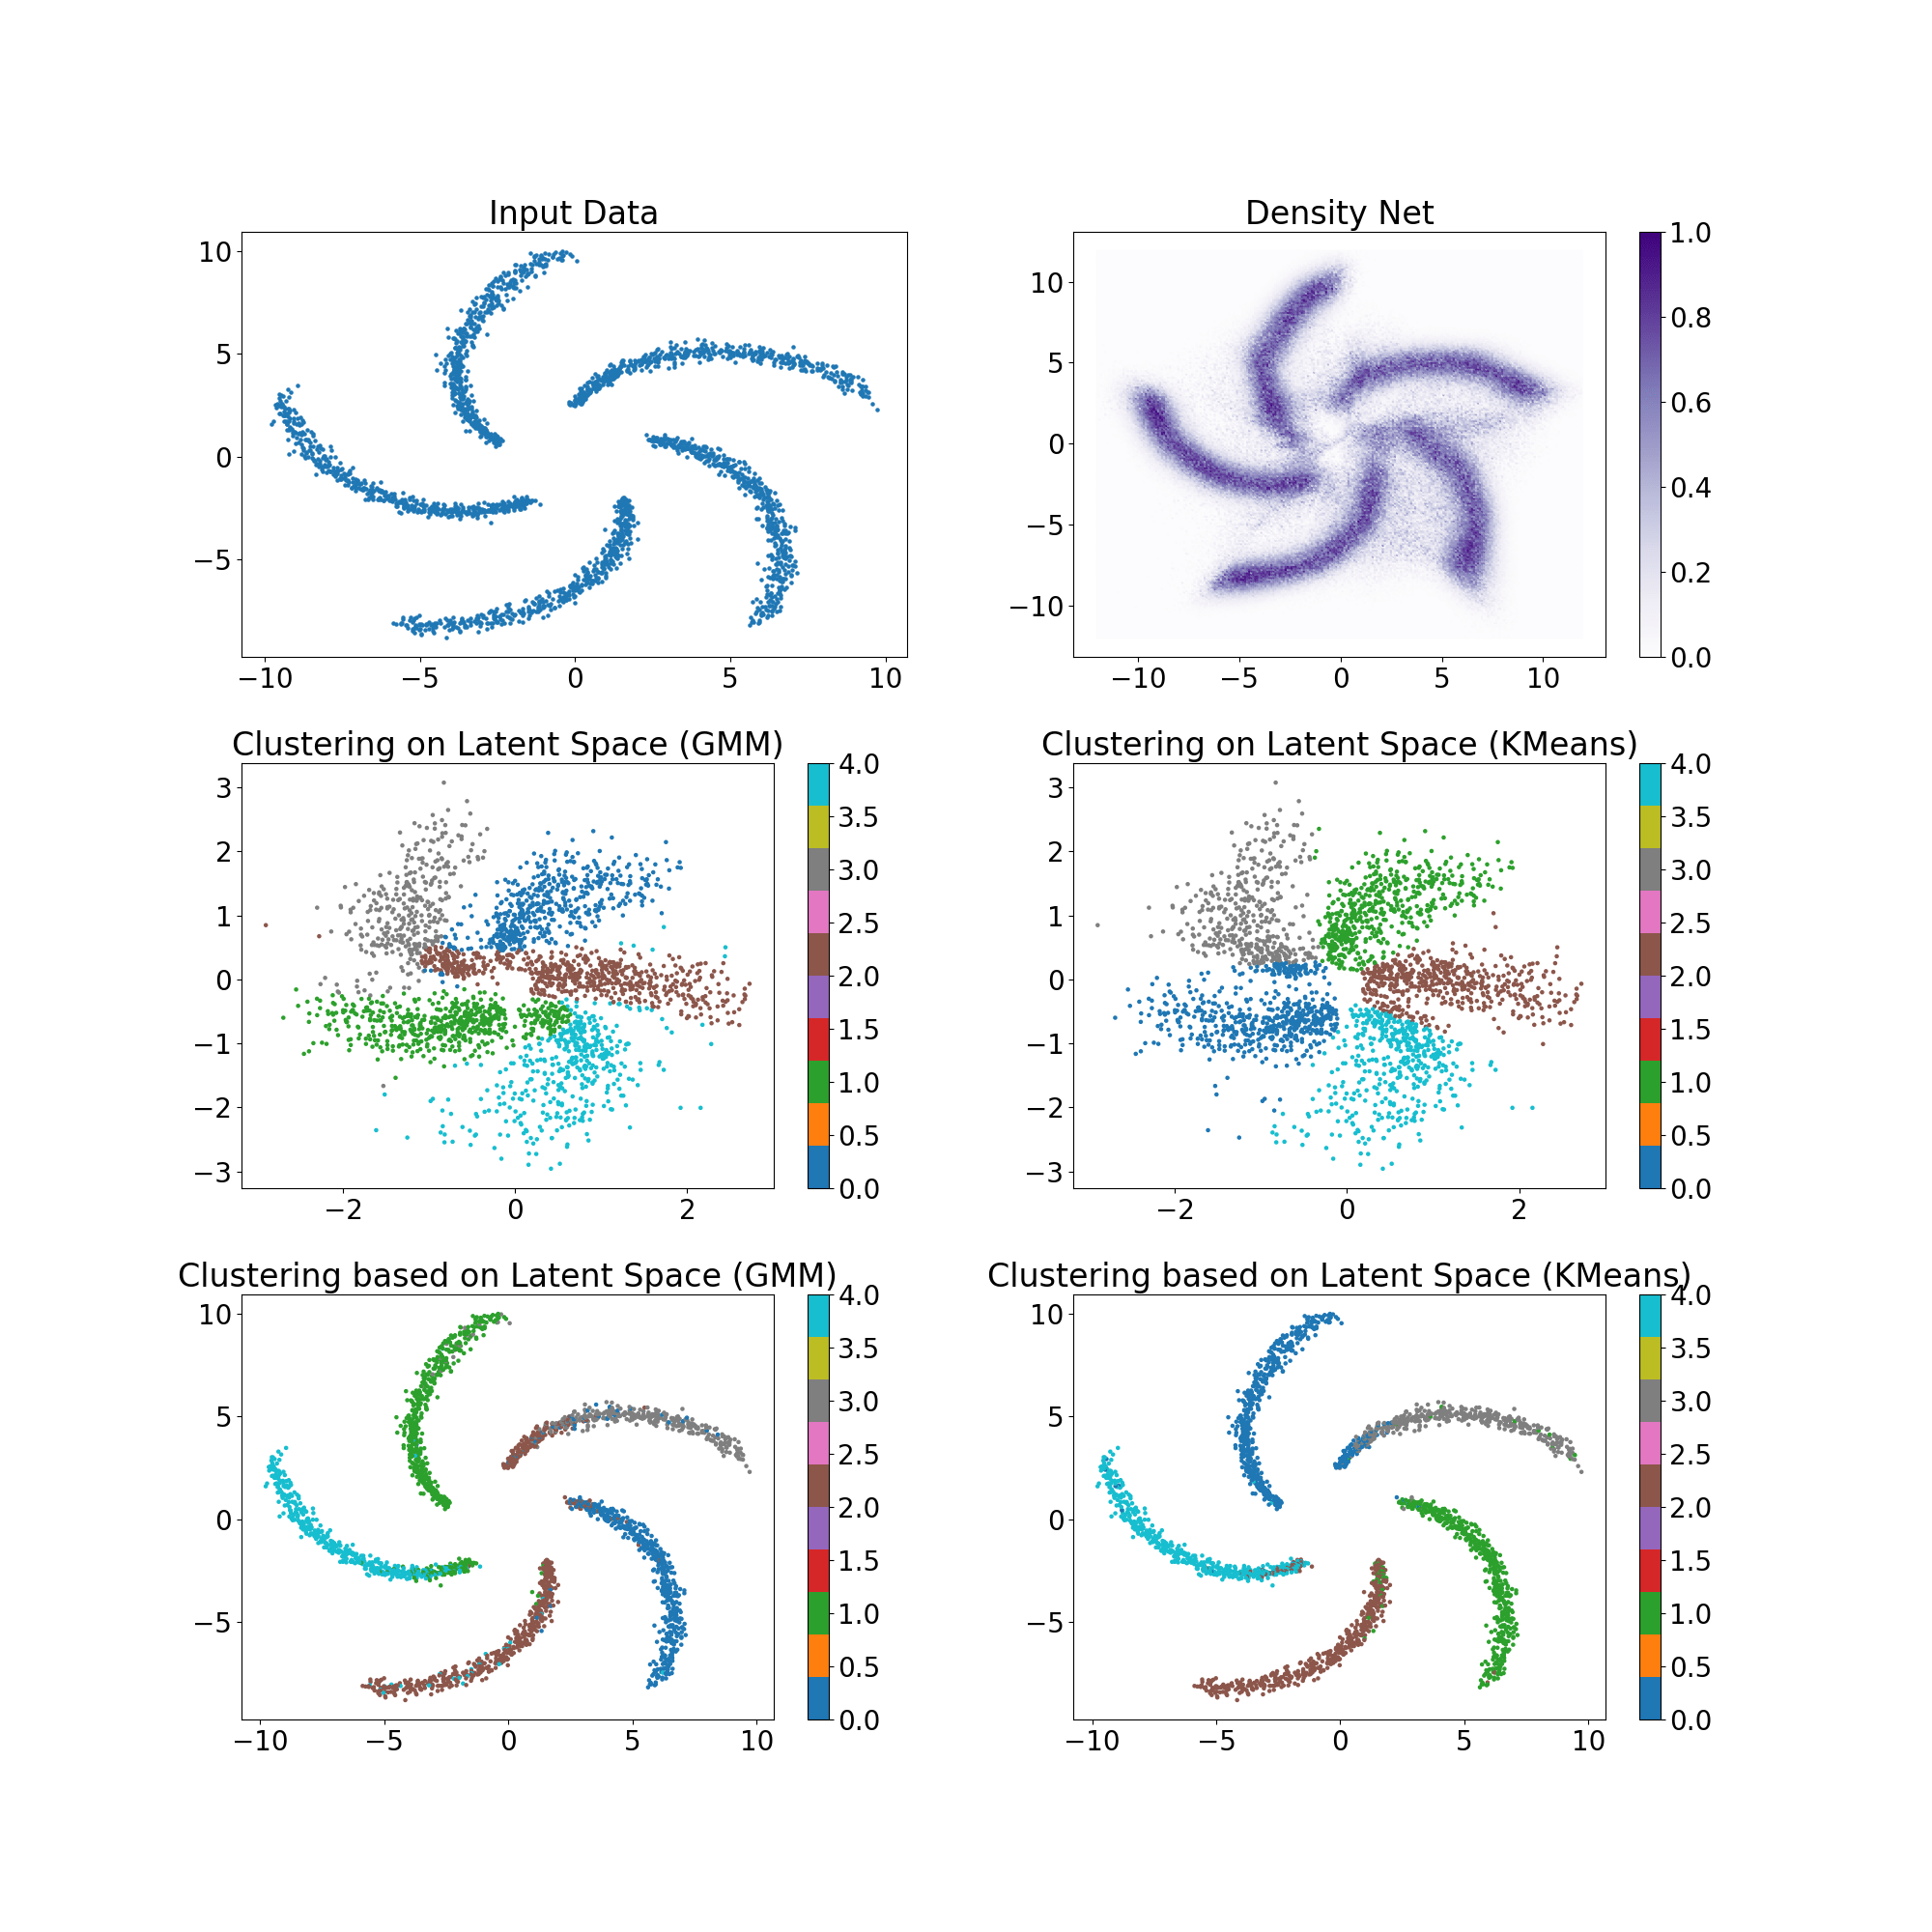
\includegraphics[trim={0 6cm 0 6cm},clip,scale=0.25]{includes/vae-clustering.png}
			\caption*{Clustering Spiral Dataset by independently clustering over VAE's latent space}
		\end{figure}

	\end{psubsection}

\clearpage

\bibliographystyle{plainnat}
\bibliography{proposal}

\end{psection}

\end{document}
